\documentclass[11pt]{article}

%% MinionPro fonts 
%\usepackage[lf]{MinionPro}
%\usepackage{MnSymbol}
\usepackage{microtype}

%% Margins
\usepackage{geometry}
\geometry{verbose,letterpaper,tmargin=1in,bmargin=1in,lmargin=1in,rmargin=1in}

%% Other packages
\usepackage{amsmath}
\usepackage{amsthm}
\usepackage[shortlabels]{enumitem}
\usepackage{titlesec}
\usepackage{soul}
\usepackage{tikz}
\usepackage{mathtools}
\usepackage{pgfplots}
\usepackage{tikz-3dplot}
\usepackage{algorithmic}
\usepackage[export]{adjustbox}
\usepackage{tcolorbox}
\usepackage{mathrsfs}
\usepackage{multicol}
\usepackage{framed}

%% Paragraph style settings
\setlength{\parskip}{\medskipamount}
\setlength{\parindent}{0pt}

%% Change itemize bullets
\renewcommand{\labelitemi}{$\bullet$}
\renewcommand{\labelitemii}{$\circ$}
\renewcommand{\labelitemiii}{$\diamond$}
\renewcommand{\labelitemiv}{$\cdot$}

%% Colors
\definecolor{rred}{RGB}{204,0,0}
\definecolor{ggreen}{RGB}{0,145,0}
\definecolor{yyellow}{RGB}{255,185,0}
\definecolor{bblue}{rgb}{0.2,0.2,0.7}
\definecolor{ggray}{RGB}{190,190,190}
\definecolor{ppurple}{RGB}{160,32,240}
\definecolor{oorange}{RGB}{255,165,0}

%% Shrink section fonts
\titleformat*{\section}{\normalsize\bf}
\titleformat*{\subsection}{\normalsize\bf}
\titleformat*{\subsubsection}{\normalsize\it}

% %% Compress the spacing around section titles
\titlespacing*{\section}{0pt}{1.5ex}{0.75ex}
\titlespacing*{\subsection}{0pt}{1ex}{0.5ex}
\titlespacing*{\subsubsection}{0pt}{1ex}{0.5ex}

%% amsthm settings
\theoremstyle{definition}
\newtheorem{problem}{Problem}
\newtheorem{example}{Example}
\newtheorem*{theorem}{Theorem}
\newtheorem*{bigthm}{Big Theorem}
\newtheorem*{biggerthm}{Bigger Theorem}
\newtheorem*{bigcor1}{Big Corollary 1}
\newtheorem*{bigcor2}{Big Corollary 2}

%% tikz settings
\usetikzlibrary{calc}
\usetikzlibrary{patterns}
\usetikzlibrary{decorations}
\usepgfplotslibrary{polar}

%% algorithmic setup
\algsetup{linenodelimiter=}
\renewcommand{\algorithmiccomment}[1]{\quad// #1}
\renewcommand{\algorithmicrequire}{\emph{Input:}}
\renewcommand{\algorithmicensure}{\emph{Output:}}

%% Answer box macros
%% \answerbox{alignment}{width}{height}
\newcommand{\answerbox}[3]{%
  \fbox{%
    \begin{minipage}[#1]{#2}
      \hfill\vspace{#3}
    \end{minipage}
  }
}

%% \answerboxfull{alignment}{height}
\newcommand{\answerboxfull}[2]{%
  \answerbox{#1}{6.38in}{#2} 
}

%% \answerboxone{alignment}{height} -- for first-level bullet
\newcommand{\answerboxone}[2]{%
  \answerbox{#1}{6.0in}{#2} 
}

%% \answerboxtwo{alignment}{height} -- for second-level bullet
\newcommand{\answerboxtwo}[2]{%
  \answerbox{#1}{5.8in}{#2}
}

%% special boxes
\newcommand{\wordbox}{\answerbox{c}{1.2in}{1cm}}
\newcommand{\catbox}{\answerbox{c}{.5in}{1cm}}
\newcommand{\letterbox}{\answerbox{c}{.7cm}{1cm}}

%% Miscellaneous macros
\newcommand{\tstack}[1]{\begin{multlined}[t] #1 \end{multlined}}
\newcommand{\cstack}[1]{\begin{multlined}[c] #1 \end{multlined}}
\newcommand{\ccite}[1]{\only<presentation>{{\scriptsize\color{gray} #1}}\only<article>{{\small [#1]}}}
\newcommand{\grad}{\nabla}
\newcommand{\ra}{\ensuremath{\rightarrow}~}
\newcommand{\maximize}{\text{maximize}}
\newcommand{\minimize}{\text{minimize}}
\newcommand{\subjectto}{\text{subject to}}
\newcommand{\trans}{\mathsf{T}}
\newcommand{\bb}{\mathbf{b}}
\newcommand{\bx}{\mathbf{x}}
\newcommand{\bc}{\mathbf{c}}
\newcommand{\bd}{\mathbf{d}}

%% LP format
%    \begin{align*}
%      \maximize \quad & \mathbf{c}^{\trans} \mathbf{x}\\
%      \subjectto \quad & A \mathbf{x} = \mathbf{b}\\
%                       & \mathbf{x} \ge \mathbf{0}
%    \end{align*}

%Space between rows:
%\def\arraystretch{2.2}
%
%Space between columns:
%\arraycolsep=1.4pt


%% Redefine maketitle
\makeatletter
\renewcommand{\maketitle}{
  \noindent SA405 -- AMP \hfill Rader \S 4.2 \\

  \begin{center}\Large{\textbf{\@title}}\end{center}
}
\makeatother

%% ----- Begin document ----- %%
\begin{document}
  
\title{Lesson 13.  Facility Location}

\maketitle

%%%
\section{Today...}

\renewcommand\labelitemi{--}
\begin{itemize}
	\item  Facility Location Introduction
	%\begin{itemize}
	%\item  General problem description
	%\item  Example Network
	%\end{itemize}
	\item  Two Variations of the Facility Location Problem
	\begin{itemize}
	\item  Set Covering Location Problem
	\item  Maximal Covering Location Problem
	%\item  (More variations in the next lesson)
%	\item  $p-$Center Problem
%	\item  $p-$Median Problem
%	\item  Fixed-Charge Location Problem
%	\item  Local $p-$Median Problem
	\end{itemize}
%	\item  Network Design Problems
%	\begin{itemize}
%	\item  Network Flow Model
%	\item  Network Design Problem
%	\end{itemize}
%	\item  Example
\end{itemize}

\section{Facility Location Introduction}
In these problems, the \textbf{input data} is...
\begin{itemize}
\item  a network of \emph{customers} (demand nodes),
\item  a set of \textbf{possible} \emph{facilities} (supply nodes),
\item  a set of edges between customers and facilities that \textbf{could} serve them
\item  distances on the edges (which could represent distance, time, cost, or some combination of these factors)
\end{itemize} 


The \textbf{goal} is to choose a set of supply facilities to serve the customers' demand based on some metric(s).
\begin{itemize}
\item For example: minimize the number of supply facilities opened while requiring that all customers are served.  
%\item The different problem types result from varied metrics and/or requirements.
\item  Real world problems of this type include locating 
\begin{itemize}
\item military installations, 
\item fire/police stations, 
\item cell phone towers, 
\item retail distribution centers and stores, 
\item schools.
\end{itemize}
\end{itemize}

%\bigskip
%\begin{tcolorbox}
%\renewcommand\labelitemi{$\circ$}
%\textbf{Basic Facility Location Assumptions:}
%\begin{itemize}
%	\item \textbf{Simple graph $G = (V, E)$}
%	\item Demand locations, $I \subseteq V$, are given
%	\item \emph{Possible} supply facility locations, $J \subseteq V$, are given
%	\begin{itemize}
%	\item[--] ($I$ and $J$ may have common nodes)
%	\end{itemize}
%	\item Edge $(i,j) \in E$ indicates that it is possible for a customer at $i$ to be supplied by a facility at $j$ (or customer at $j$ may be served by facility at $i$)
%	\begin{itemize}
%	\item[--] There is a ``distance'' $d_{c,s}$ assigned to every edge $(i,j) \in E$
%	\end{itemize}
%\end{itemize}
%\end{tcolorbox}

\newpage
\section{\emph{General} Facility Location Problems}
\begin{center}
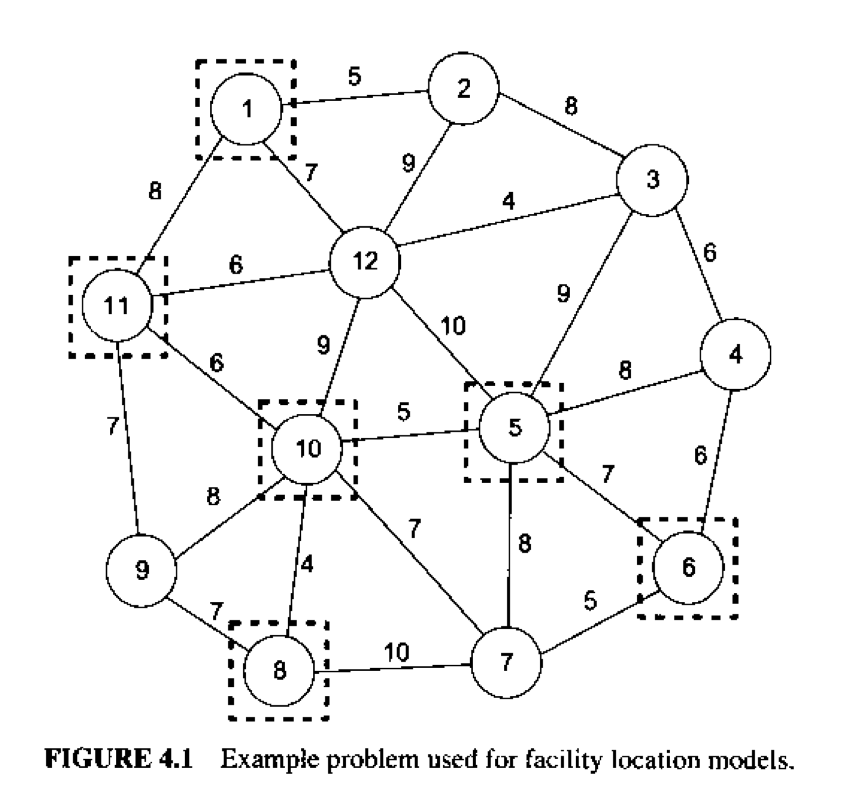
\includegraphics[width = 0.6\textwidth]{facloc}
\end{center}

\bigskip
\textbf{\emph{General} Facility Location Problem goal:}

\begin{tcolorbox}
Choose a set of supply facilities to meet customer demand according to some metric.  
\end{tcolorbox}

\bigskip
\textbf{Notation:}

Sets: 
\begin{itemize}
\item[]
 $C$ = set of customer nodes 
\item[]
$S$ = set of possible supply nodes 
\item[]
$E$ = edges $(c,s)$ connecting a customer $c$ with a supply facility $s$ that \emph{could} serve the customer
\end{itemize}

Parameters: 
\begin{itemize}
\item[]
 $d_{cs} =$ distance (or cost or time) between customer $c$ and supply location $s$, for $(c,s) \in E$
 \item[]
 $h_c =$ demand of customer $c$, for $c \in C$
\end{itemize}


\smallskip
Decision Variables: 
\begin{itemize}
\item[] 
\def\arraystretch{1.8} 
$x_s = ~\left\{ 
\begin{array}{ll} 
1 \text{ if } ~\answerbox{c}{3in}{.7cm} \\ 
0 \text{ otherwise } 
\end{array} \right. $
, for all $s \in S$
\end{itemize}

\vspace{0.5cm}
\begin{problem} We will use the network and data on the following page for all of our example problems.
\begin{enumerate}[(a)] 
\item \emph{All} vertices represent customers.  \emph{Boxed} vertices represent possible supply locations. Use set notation to list the elements of the sets $C$ and $S$.  

\answerboxone{c}{1.7cm}

\item The distance between a customer $c$ and a supplier $s$ is the length of the shortest path between them.
Find $d_{1,1}$, $d_{4,1}$, and $d_{8,5}$.  (Note that the edges in the model do not correspond directly to the edges in the graph.)

\answerboxone{c}{1cm}

\item How should the columns and rows in the distance matrix be labeled?  Do your answers in part (a) agree with the corresponding values in the distance matrix?  

\answerboxone{c}{1.5cm}
\end{enumerate}
\end{problem}

%%%%
\newpage
DATA for FACILITY LOCATION EXAMPLES:

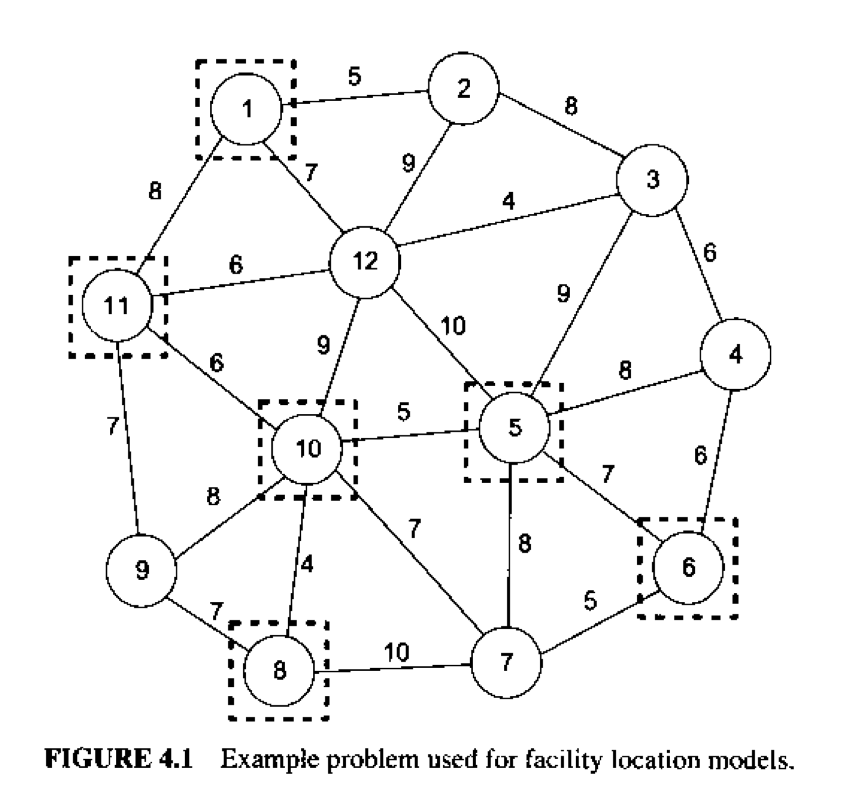
\includegraphics[width = 0.7\textwidth]{facloc}

\vfill
\includegraphics[width = 0.4\textwidth]{distances}

\vfill
$\textbf{h} = (100,~ 90,~ 110,~ 120,~ 80,~ 100,~ 95, ~75,~ 110,~ 90, ~120, ~85).$

\vfill


%%%
\newpage

\vspace{1in}
\section{\emph{Set Covering} Facility Location Problem}

\bigskip
Goal of the \textbf{set covering facility location problem}:
\begin{tcolorbox}
Open the fewest number of facilities so that every customer is ``covered'' by some facility.
\end{tcolorbox}

\bigskip
\begin{problem}
Complete the set covering facility location formulation below by adding the objective function description (1) and  the missing constraint (2).
\end{problem}

\bigskip

\begin{center}
\noindent{\textbf{Set covering facility location model}}
\end{center}

\textbf{\emph{New} Sets: }
\begin{itemize}
\item[]
$N_c = $ the facilities in $S$ that \emph{could} serve customer $\forall c \in C$
\item[] ($N_c \subseteq S$, for all $c \in C$.  $N_c$ is called the ``neighborhood'' of $c$.)
\end{itemize}


\noindent \textbf{Objective and constraint descriptions:}

(1) \answerboxone{c}{2cm}

\medskip
(2) Ensure that customer $c$ is covered by an open facility, for all $c \in C$.

    \begin{flalign}
      \minimize \quad & \sum_{s \in S} x_s  \\
      \subjectto \quad & \answerbox{c}{4cm}{1.2cm} , \text{ for all } \answerbox{c}{1.2cm}{1.2cm} \\
                       & x_s \in \{0,1\}, \text{ for } s \in S \nonumber
    \end{flalign}





%%%%
\newpage
\subsection{Example:  Set Covering Facility Location (Neighborhoods determined by distance.)}
\begin{problem}
Find the minimum number of facilities required to serve all customers.  A facility must be within $D = 9$ miles of a customer in order to serve the customer.

\begin{enumerate}[(a)]
\item For each customer $c$, the neighborhood of $N_c$ is the set of facilities that can cover customer $c$:  
\[  N_c = \left\{s \in S: ~\wordbox~\right\}, \text{ for all } c \in C.  \]
\item Complete the missing neighborhoods.   

\def\arraystretch{2.2}
\begin{multicols}{2}
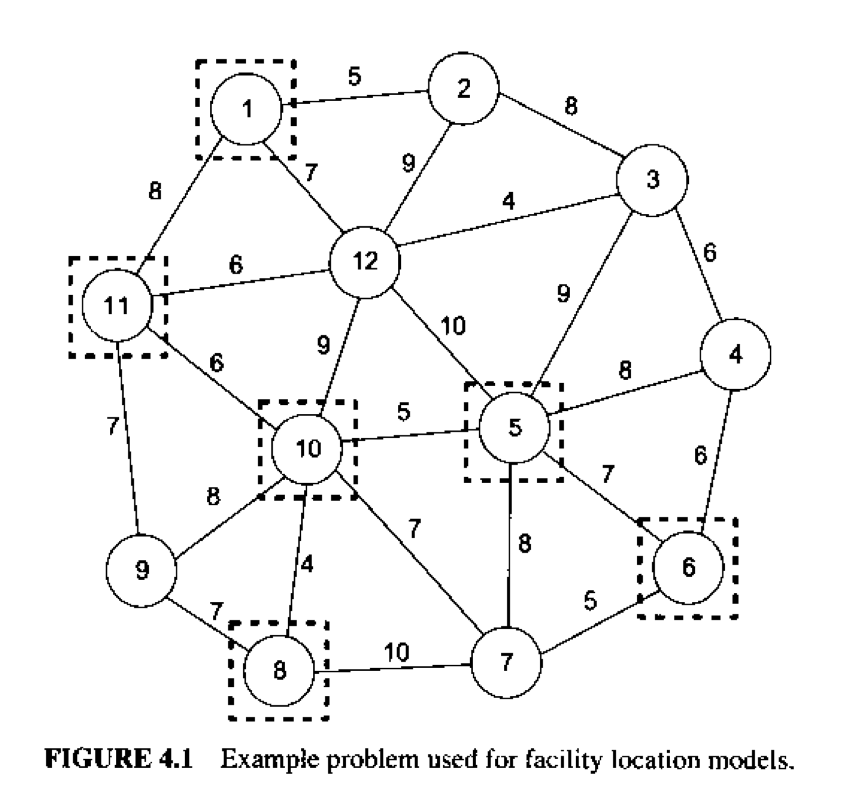
\includegraphics[width = 0.4\textwidth]{facloc}
$
\begin{array}{ll}
N_1 = \{1, 11\} \hspace{2cm} & N_7 = \{5, 6, 10\} \\
N_2 = \{1\} & N_8 = \catbox \\
N_3 = \catbox  & N_9 = \{8,10,11\} \\
N_4 = \{5,6\} & N_{10} = \catbox \\
N_5 = \{5,6,8,10\} & N_{11} = \{1,10,11\} \\
N_6 = \{5,6\} & N_{12}= \catbox \\
\end{array}
$
\end{multicols}
\item  How many facilities are required?  List the values of the decision variables that correspond to an optimal feasible solution.

\answerboxone{c}{1cm}

\item Write an abbreviated version of the concrete model.

\answerboxone{c}{6.3cm}
\end{enumerate}
\end{problem}

%%%%
\newpage
\section{\emph{Maximal Covering} Location Problem}
The goal of the \textbf{maximal covering location problem}:
\begin{tcolorbox}
Select the $p$ facilities to open in order to maximize the customer demand that is covered.  (A customer, $c$, can only be covered by a supply facility, $s$, in its neighborhood: $s \in N_c$.)
\end{tcolorbox}


\bigskip
\begin{problem}
Complete the maximal covering facility location formulation below by adding the objective function (3),  the missing constraint (4), and the description for constraint (5).
\end{problem}
\bigskip


\begin{center}
\noindent{\textbf{Maximal covering facility location model}}
\end{center}

\textbf{
\emph{New} Parameters: }
\begin{itemize}
\item[] $h_c = $ the demand at customer $c$, for all $c \in C$
\item[]  $p = $ the number of facilities to open
\end{itemize}

\textbf{\emph{New} Decision Variables: }
\begin{itemize}
\item[] \def\arraystretch{1.8} $y_c = ~\left\{ \begin{array}{ll} 1 \text{ if a facility $s$ in the neighborhood of $c$ has been selected} \\ 0 \text{ otherwise } \end{array} \right. $
, for all $c \in C$
\end{itemize}

\textbf{Objective and constraint descriptions:} 

(3) Maximize the total customer demand that is covered. % \answerboxone{c}{1cm}

(4) Ensure that exactly $p$ facilities are opened.

(5) \answerboxone{c}{1.7cm}

    \begin{align}
      \maximize \quad & \answerbox{c}{4cm}{1.2 cm} \\ %\sum_{c\in C} h_c y_c  \\
      \subjectto \quad  &  \answerbox{c}{4cm}{1.2 cm} \\  %\sum_{s \in S} x_s = p \\
					& \sum_{s \in N_c} x_s \geq y_c, \text{ for } c \in C \\
                       & x_s \in \{0,1\}, \text{ for } s \in S \nonumber\\
                       & y_c \in \{0,1\}, \text{ for } c \in C \nonumber
    \end{align}

%%%%
\newpage
\subsection{Example:  Maximal Covering Facility Location Problem}

\begin{problem}
We saw in the last example that every customer's demand can be met by three facilities.  Suppose that we can only afford to build and maintain $p = 2$ facilities, and the demand values for the customers (in order) are 
\[
\textbf{h} = (100, 90, 110, 120, 80, 100, 95, 75, 110, 90, 120, 85).
\]
Opening which two facilities will allow us to cover the most total customer demand?
\end{problem}

\bigskip

\begin{enumerate}[(a)]
\item The optimal solution is to choose facilities 5 and 11.  List the values of the decision variables $x_s$ and $y_c$ in the optimal solution.  Illustrate the solution on the graph of the network.

\hfill 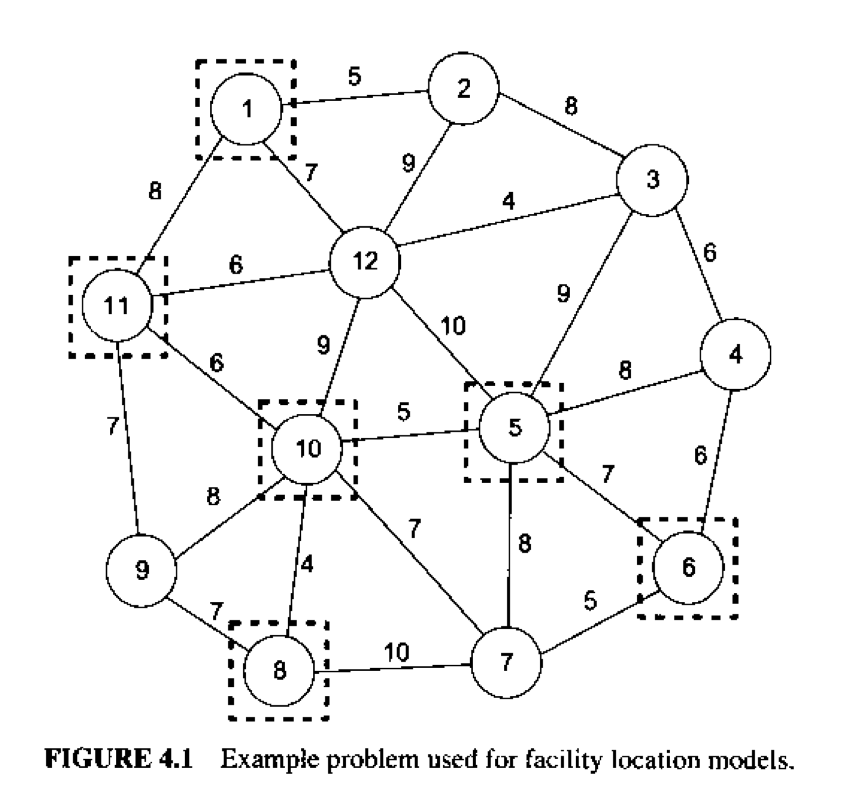
\includegraphics[width = 0.4\textwidth]{facloc}

\item Find the optimal objective function value.  What does it mean?
	
\answerboxone{c}{1cm}

\item Write concrete versions of the following:
\begin{enumerate}[i]
\item objective function:

\answerboxtwo{c}{1cm}

\item constraint (4):

\answerboxtwo{c}{1cm}

\item constraints (5) for customers 4 and 8:

\answerboxtwo{c}{2cm}
\end{enumerate}
\end{enumerate}


\end{document}



%%%%
\newpage
\section{\emph{$p$-Center} Facility Location Problem:  Minimize Maximum Distance}

Goal of the \textbf{$p$-center problem}:
\begin{tcolorbox}
Choose $p$ supply facilities to open in order to minimize the maximum distance between any customer and the supply facility that serves it.
\end{tcolorbox}

\emph{New} Decision Variables: 
\begin{itemize}
\item[] \def\arraystretch{1.8} $z_{c,s} = ~\left\{ \begin{array}{ll} 1 \text{ if ``open'' facility $s$ is assigned to serve customer $c$ }  
\\ 0 \text{ otherwise } \end{array} \right. $
, for all $c \in C,~ s \in S$
\item[] $W = $ the maximum distance between a customer and the facility chosen to serve it
\end{itemize}
\emph{Notice that by the way $z_{c,s}$ is defined, we assume that each customer could be served by any supplier.}
%\vspace{-.2ztcm}
    \begin{align}
      \minimize \quad & W  \\
      \subjectto \quad 
 				          & \sum_{s \in S} z_{c,s} = 1, \text{ for } c \in C \\
 					   & \sum_{s \in S} d_{c,s}z_{c,s} \leq W, \text{ for } c \in C \\		     	                             & z_{c,s} \leq x_s, \text{ for } c \in C,~s \in S \\
     	                             & \sum_{s \in S} x_s = p \\
                       & x_s \in \{0,1\}, \text{ for } s \in S \nonumber\\
                       & z_{c,s} \in \{0,1\}, \text{ for } c \in C, ~s \in S \nonumber
    \end{align}

\begin{problem}  Explain the purpose of the objective function and each numbered constraint.

\bigskip
(6) and (8) \answerbox{c}{13.9cm}{2cm}

(7) \answerboxone{c}{1.7cm}

(9) \answerboxone{c}{1cm}

(10) \answerboxone{c}{1.7cm}

\end{problem}

%%%%
\newpage
\subsection{Example:  $p$-Center Facility Location Problem}

\begin{problem}
Assume the same network, distances, and demand values that we have already been using.  We wish to find the
$p=2$ facilities that can serve all of the customers so that the maximum distance between a customer and the facility it is served by is minimized.
\end{problem}

\begin{enumerate}[(a)]
\item Again, the optimal solution is to choose facilities 5 and 11. Facility 5 serves the customers 3, 4, 6, 7, and 8.  Facility 11 serves the rest.  Write the values of the decision variables for this optimal solution and draw the solution on the network.

\hfill 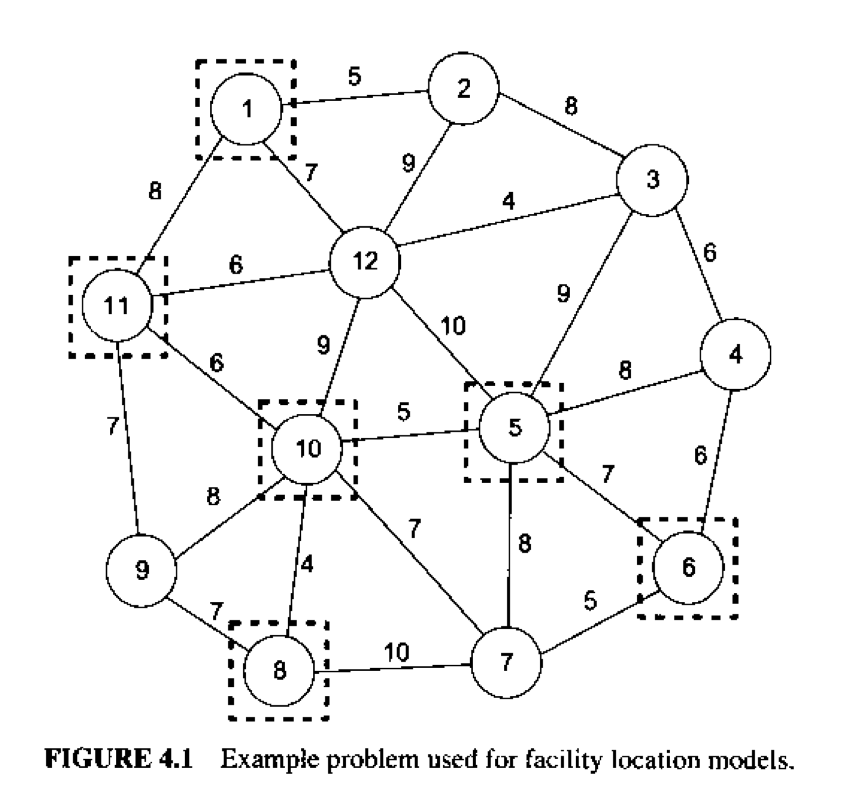
\includegraphics[width = 0.4\textwidth]{facloc}

\item Find the optimal objective function value.  What does it mean?

\answerboxone{c}{1.7cm}
\item Write concrete versions of the following:
\begin{enumerate}[i]
\item constraint (7) for customers 5 and 12:

\answerboxtwo{c}{1.7cm}

\item constraint (8) for customers 5 and 12:

\answerboxtwo{c}{1.7cm}

\item constraints (9) for supplier 5 and all of its potential customers:

\answerboxtwo{c}{1.7cm}
\end{enumerate}
\end{enumerate}

%%%%
\newpage
\section{\emph{$p$-Median} Facility Location Problem: Minimize Total Distance}
Goal of the \textbf{$p$-median problem}:
\begin{tcolorbox}
Choose exactly $p$ supply facilities to open to minimize the \emph{total} distance \emph{weighted by customer demand}, between customers and the facilities that serve them.
\end{tcolorbox}

%\emph{New} Parameters: 
%\begin{itemize}
%\item[] $h_c = $ the demand at customer $i$, for all $c \in C$
%\end{itemize}
%
%\emph{New} Decision Variables: 
%\begin{itemize}
%\item[] \def\arraystretch{1.8} $y_{c,s} = ~\left\{ \begin{array}{ll} 1 \text{ if } \hspace{3in} \\ 0 \text{ if } \end{array} \right. $
%, for all $c \in C,~ s \in S$
%\end{itemize}


    \begin{align}
      \minimize \quad & \sum_{c \in C} \sum_{s \in S} h_c d_{c,s} z_{c,s}  \\
      \subjectto \quad & \sum_{s \in S} z_{c,s} = 1, \text{ for } c \in C \\
      	                             & \sum_{s \in S} x_s = p \\
      	                             & z_{c,s} \leq x_s, \text{ for } c \in C,~s \in S \\
                       & x_s \in \{0,1\}, \text{ for } s \in S \nonumber\\
                       & z_{c,s} \in \{0,1\}, \text{ for } c \in C, ~s \in S \nonumber
    \end{align}

\bigskip
\begin{problem}
Explain the purpose of the objective function and each numbered constraint.
\end{problem}

(11) \answerboxone{c}{2.5cm}

(12) Every customer is served.

(13) Exactly $p$ facilities are opened.

(14) \answerboxone{c}{2.5cm}


%%%%
\newpage
\subsection{Example: $p$-Median Facility Location Problem}

\begin{problem}
Using the same data, now we wish to choose $p = 2$ facilities to open in order to minimize the total weighted distance between customers and the facilities that serve them.
\end{problem}

\begin{enumerate}[(a)]
\item The optimal solution is to choose facilities 6 and 11.  Facility 6 satisfies the demands of customers 4, 5, 6, and 7.  Facility 11 serves the rest of the customers.  Illustrate the solution on the graph.

\begin{center} 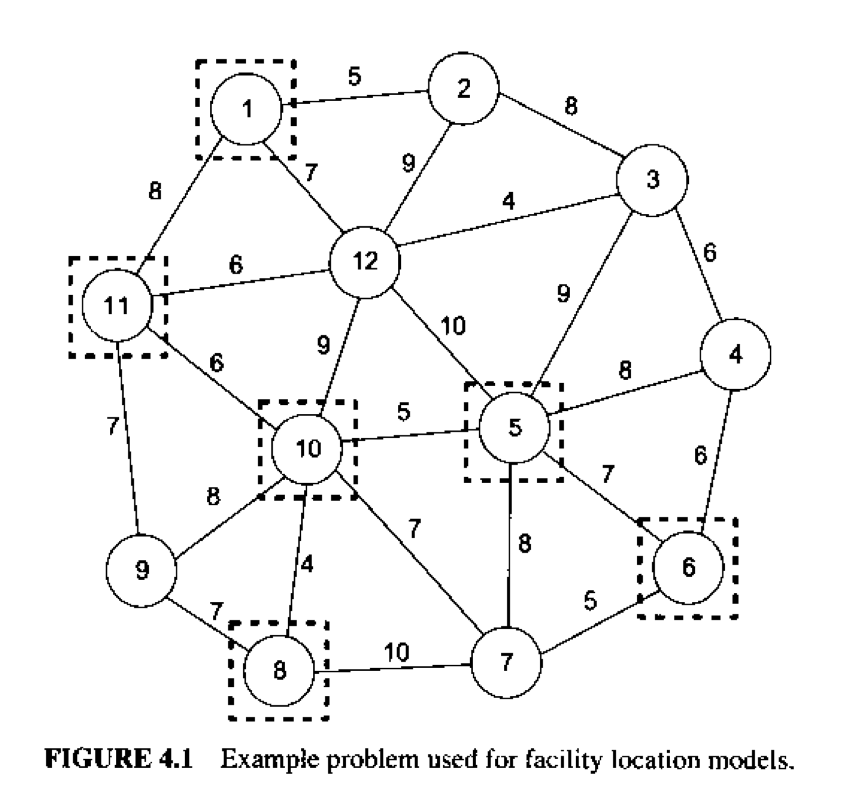
\includegraphics[width = 0.4\textwidth]{facloc} \end{center}

\item Find the optimal objective function value.  What does it mean?
	
\answerboxone{c}{2cm}

\item Write concrete versions of the following:
\begin{enumerate}[i]
\item objective function (abbreviated)

\answerboxtwo{c}{1.7cm}

\item constraint (12) for customers 6 and 7:

\answerboxtwo{c}{1.7cm}

\item constraints (14) for supplier 10 and all of its potential customers:

\answerboxtwo{c}{1.7cm}
\end{enumerate}

\end{enumerate}

%%%%
\newpage

\section{\emph{Fixed-Charge} Location Problem}

This is a more general purpose model.

\bigskip
Goal of the \textbf{fixed-charge location problem}.

\begin{tcolorbox}
Each facility has a fixed-charge cost for opening, as well as a maximum capacity.  There is also a \emph{per unit demand per unit distance} shipping cost.

\smallskip
The goal is to
choose $p$ facilities to open so that total cost (facility opening + shipping) of meeting all demand is minimized without exceeding facility capacities.
\end{tcolorbox}

\emph{New} Parameters: 
\begin{itemize}
\item[] $f_s = $ the fixed-charge cost of opening facility $s$, for all $s \in S$ 
\item[] $cap_s = $ capacity of facility $s$, for all $s \in S$ 
\item[]  $\alpha = $ shipping cost per unit demand, per unit distance
\end{itemize}

%\emph{New} Decision Variables: 
%\begin{itemize}
%\item[] \def\arraystretch{1.8} $y_{c,s} = ~\left\{ \begin{array}{ll} 1 \text{ if } \hspace{3in} \\ 0 \text{ if } \end{array} \right. $
%, for all $c \in C,~ s \in S$
%\end{itemize}


    \begin{align}
      \minimize \quad & \sum_{s \in S} f_s x_s + \alpha \sum_{c \in C} \sum_{s \in S} h_c d_{c,s} z_{c,s}  \\
      \subjectto \quad & \sum_{s \in S} z_{c,s} = 1, \text{ for } c \in C \\
      	                             & \sum_{s \in S} x_s = p \\
      	                             & \sum_{c \in C} h_c z_{c,s} \leq cap_s x_s, \text{ for } s \in S \\
                       & x_s \in \{0,1\}, \text{ for } s \in S \nonumber\\
                       & z_{c,s} \in \{0,1\}, \text{ for } c \in C, ~s \in S \nonumber
    \end{align}

\begin{problem}
Explain the purpose of the objective function and each numbered constraint.

\smallskip
(15) Minimize total cost:  facility opening costs + shipping costs

(16) Every customer must be served by exactly one facility

(17) Exactly $p$ facilities are opened

(18) \answerboxone{c}{2.7cm}
\end{problem}

%%%%
\newpage
\subsection{Example: Fixed-Charge Facility Problem}

\begin{problem}
Use the same network, distances, and demands.  Also, $\alpha = 1$ is the per unit demand per unit distance shipping cost.  
The fixed costs for opening facilities are
\[
f= (5000,~7000,~6000,~4000,~7000,~12000),
\]
and the facility capacities are
\[
C = (600,~650,~600,~500,~650,~800).
\]
We wish to find the $p=2$ facilities to open which will minimize the total facility opening and shipping costs of the network, without exceeding facility capacities.
\end{problem}


\begin{enumerate}[(a)]
\item The optimal solution is to choose facilities 1 and 6.  Facility 1 satisfies the demands of customers 1, 2, 9, 10, 11, and 12.  Facility 6 serves the rest of the customers.  Illustrate the solution on the graph.

\begin{center} 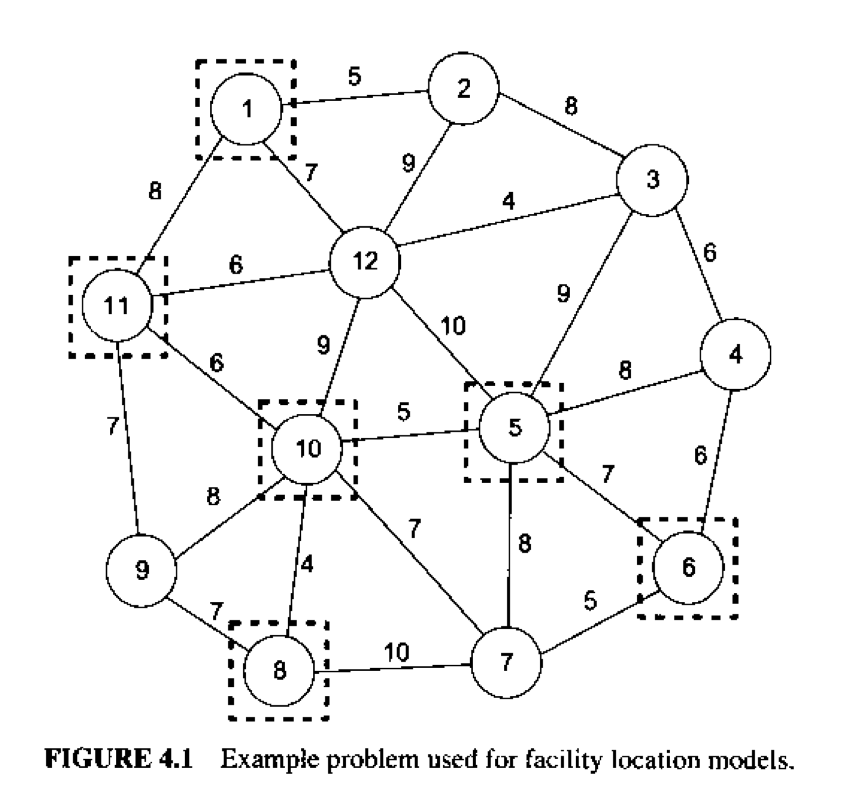
\includegraphics[width = 0.4\textwidth]{facloc} \end{center}

\item Find the optimal objective function value.  What does it mean?
	
\answerboxone{c}{1.8cm}

\item Write concrete versions of the following:
\begin{enumerate}[i.]
\item objective function (abbreviated)

\answerboxtwo{c}{1.7cm}

\item constraint (18) for supply facility 6:

\answerboxtwo{c}{1.7cm}

\end{enumerate}
\end{enumerate}

%%%%





\end{document}




\end{document}